\documentclass[varwidth=true, border=2pt]{standalone}

\usepackage{pgfplots}
\usepackage{tikz}
\usetikzlibrary{patterns}

    \tikzset{
        hatch distance/.store in=\hatchdistance,
        hatch distance=10pt,
        hatch thickness/.store in=\hatchthickness,
        hatch thickness=2pt
    }

    \makeatletter
    \pgfdeclarepatternformonly[\hatchdistance,\hatchthickness]{flexible hatch}
    {\pgfqpoint{0pt}{0pt}}
    {\pgfqpoint{\hatchdistance}{\hatchdistance}}
    {\pgfpoint{\hatchdistance-1pt}{\hatchdistance-1pt}}%
    {
        \pgfsetcolor{\tikz@pattern@color}
        \pgfsetlinewidth{\hatchthickness}
        \pgfpathmoveto{\pgfqpoint{0pt}{0pt}}
        \pgfpathlineto{\pgfqpoint{\hatchdistance}{\hatchdistance}}
        \pgfusepath{stroke}
    }

\begin{document}
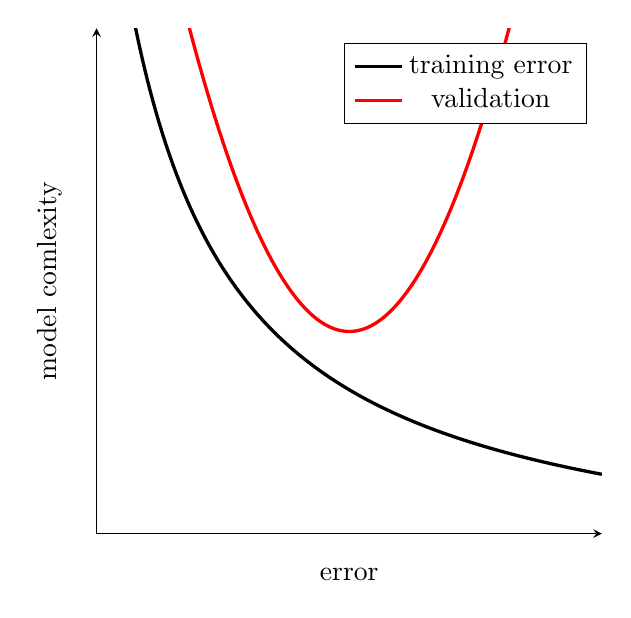
\begin{tikzpicture}
    \begin{axis}[
        legend pos=north east,
        axis x line=middle,
        axis y line=middle,
        width=8cm,
        height=8cm,
        %grid style={dashed, gray!30},
        xmin= 0,     % start the diagram at this x-coordinate
        xmax= 2,    % end   the diagram at this x-coordinate
        ymin= 0,     % start the diagram at this y-coordinate
        ymax= 2,   % end   the diagram at this y-coordinate
        xlabel=error,
        ylabel=model comlexity,
        ticks=none,
        xticklabels={,,},
        yticklabels={,,},
        x label style={at={(axis description cs:0.5,-0.05)},
                       anchor=north},
        y label style={at={(axis description cs:-0.05,0.5)},
                       anchor=south,
                       rotate=90},]
      % plot it
      \addplot[domain=-0.29:2,samples=500,very thick] {1/(x+0.3)-0.2};
      \addplot[domain=0:2, red, very thick,samples=500] {3*(x-2)*x+3.8};
      \addlegendentry{training error}
      \addlegendentry{validation}
    \end{axis}
\end{tikzpicture}
\end{document}
